 While on-site assertion of an intersection is plausible, the scope of a single observer is limited, as one can only keep track of 
 so many cyclists at once. Likewise with analyzing recorded video footage, while not bound by time, is still a time-consuming process, 
 especially as the views of cyclists can be obstructed by other passing vehicles or permanent fixtures.
\ \\

\raggedbottom
\noindent
\begin{tabular}{@{}cc}
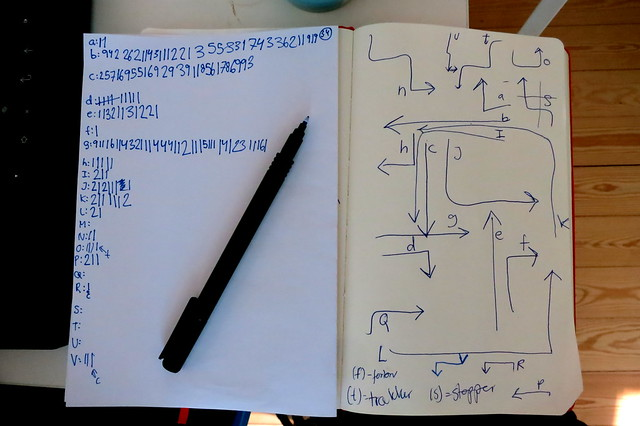
\includegraphics[width=1.0\columnwidth]{desire_line_counts} 
\end{tabular}
\captionof{figure}{Manual desire line counts (Copenhagenize, 2014)}
\

The latter issue of keeping track of unique cyclists as their view is temporally obstructed is one also faced by 
object tracking algorithms in video. In theory, a top-down overhead view, overlooking from the center of the intersection would be optimal for minimizing obstruction.
However, the height required for such a recording setup as well as the lack of permanent fixtures makes this approach very impractical. 
Current state-of-the-art object detection algorithms (e.g.~YOLO) also perform worse at categorizing objects, especially bicycles, 
using an overhead view compared to a semi-frontal view. We therefore propose deploying a multi-camera setup, overlooking an intersection from
multiple sides.
\ \\

A top-level areal view can help identify rule compliance through the intersection by comparing
the shares of cyclists using chosen desire lines to reach the same destination. 
To bring nuance to the analysis, one can dig into the footage to assess the behavior of 
each identified cyclist using a specific desire line. 
This can provide insights about the context to non-intended behavior such as state of traffic signals, 
vehicles and the momentum of other cyclists.